\documentclass{tufte-handout}

%\geometry{showframe}% for debugging purposes -- displays the margins

\usepackage{amsmath}

% Set up the images/graphics package
\usepackage{graphicx}
\setkeys{Gin}{width=\linewidth,totalheight=\textheight,keepaspectratio}
\graphicspath{{graphics/}}

\title{Endocrine Control of Growth}
\author{Dave Bridges, Ph.D.}
%\date{24 January 2009}  % if the \date{} command is left out, the current date will be used

% The following package makes prettier tables.  We're all about the bling!
\usepackage{booktabs}

% The units package provides nice, non-stacked fractions and better spacing
% for units.
\usepackage{units}

% The fancyvrb package lets us customize the formatting of verbatim
% environments.  We use a slightly smaller font.
\usepackage{fancyvrb}
\fvset{fontsize=\normalsize}

% Small sections of multiple columns
\usepackage{multicol}

% Provides paragraphs of dummy text
\usepackage{lipsum}

% These commands are used to pretty-print LaTeX commands
\newcommand{\doccmd}[1]{\texttt{\textbackslash#1}}% command name -- adds backslash automatically
\newcommand{\docopt}[1]{\ensuremath{\langle}\textrm{\textit{#1}}\ensuremath{\rangle}}% optional command argument
\newcommand{\docarg}[1]{\textrm{\textit{#1}}}% (required) command argument
\newenvironment{docspec}{\begin{quote}\noindent}{\end{quote}}% command specification environment
\newcommand{\docenv}[1]{\textsf{#1}}% environment name
\newcommand{\docpkg}[1]{\texttt{#1}}% package name
\newcommand{\doccls}[1]{\texttt{#1}}% document class name
\newcommand{\docclsopt}[1]{\texttt{#1}}% document class option name

%line break in cell
\newcommand{\specialcell}[2][c]{%
  \begin{tabular}[#1]{@{}c@{}}#2\end{tabular}}

\begin{document}

\maketitle% this prints the handout title, author, and date

\begin{abstract}
\noindent This lecture covers endocrine control of growth.  The primary hormone that mediates growth is, unsurprisingly known as growth hormone\sidenote{sometimes refered to as somatorop(h)in, hGH, or when generated recombinantly rhGH}.  This lecture covers the following pages in the textbook: 350-353 and 358-359 \cite{Widmaier2013}.
\end{abstract}

\tableofcontents

\pagebreak

\section{Learning Objectives}
For this lecture, the learning objectives are:
\begin{itemize}
\item List the hormones important for growth at key times in a person's life.
\item Describe the functions of human growth hormone on growth (bones and soft tissues), and on metabolism, and the regulation of its secretion.  Explain what 'rhGH' means.
\item State the "dual effector hypothesis" for GH actions, and the relative roles of GH and IGF-1 in growth control. 
\item Describe the interactions among all the key growth-regulating hormones at key times of a person's life: in utero, neonatally, childhood, puberty, adulthood, and senescence.
\item Describe the daily regulation of GH levels and the physiological relevance of these cycles.

\end{itemize}

\pagebreak

There are several hormones that are involved in normal growth.  The most important is growth hormone, but insulin, thyroid hormones, cortisol, Vitamin D and sex hormones are also very important.  These are covered in separate lectures.  Generally proper growth (length and mass increase) requires proper nutrition\sidenote{both macro- and micronutrients} and a good psychosocial environment.   This requires the integration of many signals.

\newthought{Humans undergo two major growth phases.}  During the first two years there is a dramatic increase in bone, muscle and other organ size.  The second major growth phase, which occurs during puberty is at 12-20 years old.  Sex hormones\sidenote{estrogen and testosterone} cause this growth spurt by increasing the levels of both GH\sidenote{Growth hormone, or when generated recombinantly known as rhGH.} and IGF-1\sidenote{Insulin-like growth factor-1.}.  The hormones required at each stage are shown in Table \ref{tab:hormone-requirements}.  Vitamin D and the thyroid hormones will be discussed in future lectures.

\begin{table}
  \centering
  \begin{tabular}{lll}
    \toprule
Stage & Age & Hormonal Requirements \\
\midrule
Prenatal & (9 months) & Insulin \\
Infantile & 0-1 & Insulin \\
Juvenile & 1-12 years & GH, Insulin, T$_3$, Vitamin D \\
Adolescent  & \specialcell[t]{10-14 (F) \\ and 12-16 (M)} & \specialcell[t]{GH, insulin, T$_3$, Vitamin D \\ and Sex Steroids} \\
Adult & Puberty - 100 & Normally limited growth \\
    \bottomrule
  \end{tabular}
  \caption{Hormones required at different stages of growth.}
  \label{tab:hormone-requirements}
  %\zsavepos{pos:normaltab}
\end{table}


\section{Regulation of Growth Hormone and IGF-1 Levels}

The main regulator of growth are GH and IGF-1.  IGF-1 is regulated by GH, similar to the way that ACTH can promote the release of cortisol.  The primary difference is that \emph{both} GH and IGF-1 have important peripheral functions\sidenote{This is known as the \emph{dual-effector hypothesis}, which means that you require both GH and IGF-1 to be functional to see the effects of growth hormone}.  These hormones are under control of the hypothalamus and pituitary.

\subsection{Hypothalamic and Pituitary Control of Growth Hormone}

Growth hormone is released from the somatotroph cells in the anterior pituitary.  The somatotrophs secrete growth hormone into the circulation upon PKA activation.  The two primary regulators of GH secretion are the hypothalamic hormones GHRH\sidenote{growth hormone releasing hormone.} and somatostatin\sidenote{Sometimes called growth hormone inhibiting hormone or GHIH.} which can both be secreted into the hypophyseal portal system from the hypothalamus.  The GPCR receptors of these hormones are Gs and Gi linked receptors respectively, so either promote or inhibit the activation of PKA.  This process is summarized in Figure \ref{fig:gh-igf1}.


\begin{marginfigure}
  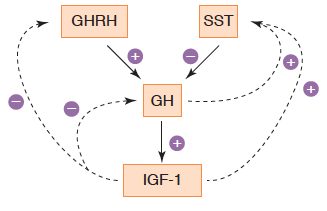
\includegraphics{figures/gh-igf1}
  \caption{Regulation of GH and IGF-1 levels.}
    \label{fig:gh-igf1}
\end{marginfigure}

\newthought{Growth hormone is highest during youth while people are actively growing.}  As a person ages, the amount of growth hormone decreases.  This is primarily due to decreases in GHRH secretion from the hypothalamus and not due to an insensitivity of cells to GHRH, GH or IGF-1.  Growth hormone also undergoes a normal diurnal rhythm.  GH levels are highest shortly after going to sleep and lower during the day.  Because of this, most growth occurs during sleeping when nutrients can be used for growth and are not needed for normal activities.

\subsection{Growth Hormone Regulates IGF-1 Secretion}

While growth hormone has some effects on growth, several important effects are mediated by another hormone IGF-1\sidenote{insulin-like growth factor 1}, whose expression is regulated by growth hormone.  IGF-1 is a protein hormone synthesized and released primarily from the liver and signals through receptor tyrosone kinases.  In addition to regulation by growth hormone, IGF-1 can also be regulated by nutrient status, such that if a person is starving, IGF-1 levels are low, even if GH levels are elevated.


\section{Effects of Growth Hormone}

The main role of the GH/IGF-1 axis is to encourage muscle, bone and other organ growth and to divert important nutrients such as proteins, carbohydrates and lipids towards that end.  As such, GH/IGF-1 has catabolic actions in storage depots such as adipose tissue, but anabolic actions in growing bones and muscles.  In this way GH/IGF-1 function both anabolically (in growing muscle and bone) and catabolically (in storage tissues).

\subsection{Growth Hormone and IGF-1 Signaling}

GH functions through a receptor\sidenote{The Growth Hormone Receptor.} of the JAK/STAT family.  These receptors function primarily by phosphorylating a class of transcription factors known as STATs\sidenote{Signal Transducer and Activator of Transcription.   For GH signaling, the most important is STAT5.} which then produce new mRNAs by binding to specific DNA binding sites on promoters of those genes.  IGF-1 on the other hand functions through a receptor tyrosine kinase, similar to insulin.  This can result in rapid activation of enzymes that are important for distributing nutrients towards growing tissues.

\subsection{Bone and Soft Tissue Growth}

Bones grow via expansion of a region known as the epiphysial growth plate.  A specialized cell type known as osteoblasts form bone at the edge of the plate in concert with chondrocytes, which lay down cartilage in the interior.  This is shown in Figure \ref{fig:bone-growth}.  The surge of sex hormones in puberty assists in the closing of the epiphysial growth plate, preventing further bone growth in adulthood.

\begin{figure}
\centering
  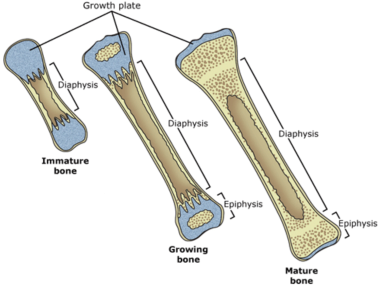
\includegraphics[width=0.8\textwidth]{figures/bone-growth}
  \caption{Growth of bone from the growth plate.}
    \label{fig:bone-growth}
\end{figure}


\newthought{Muscle growth occurs primarily via two mechanisms, the induction of protein synthesis and the generation of new muscle cells\sidenote{This is known as myogenesis.}}  Both of these processes are primarily controlled by IGF-1, which activates a nutrient sensing protein kinase called mTORC1\sidenote{mechanistic target of rapamycin complex 1}.  The signaling pathway by which IGF-1 activates mTORC1 is very similar to the insulin signaling pathway we will discuss in the lecture on the pancreas and insulin action.  Once activated mTORC1 mediates both myogenesis and muscle growth.

\subsection{Regulation of Metabolism}

In addition to promoting protein synthesis in muscle, GH/IGF-1 signaling has several other important peripheral effects.  In order to provide substrates for bone and soft tissue growth, GH induces liver gluconeogenesis and promotes lipid breakdown in adipose tissue, to provide substrates for further gluconeogenesis\sidenote{Both cortisol and growth hormone promote gluconeogenesis, but they get the precursors from different substrates.  Think about how the source of substrates can differ, and what the repercussions and function of these differences are.}.  To allow for glucose to enter the muscle, IGF-1 stimulates glucose uptake in muscle and promotes glycogen and lipid storage in these tissues.  The mechanism for this is the same as insulin action, which will be discussed in the lecture on pancreatic function.

\section{Integration of GH with Other Endocrine Factors}

Several other hormones work with, or against GH  to regulate growth.  As stated above, nutrient status is extremely important for growth hormone signaling but insulin and thyroid hormones also enhance GH signaling.  These are summarized in Table \ref{tab:hormone-interactions}

\begin{table}
  \centering
  \begin{tabular}{ll}
    \toprule
Hormone & Effects \\
\midrule
Insulin & \specialcell[t]{Fetal Growth \\ IGF-1 Secretion \\ Protein Synthesis} \\
Thyroid Hormone & \specialcell[t]{GH Production \\ CNS Development} \\
\specialcell[t]{Testosterone  \& \\ Estrogen} & \specialcell[t]{GH Secretion at puberty \\ Eventual epiphysial closure \\ protein synthesis (T)} \\
Cortisol & \specialcell[t]{Inhibits growth hormone release \\ Protein catabolism} \\
    \bottomrule
  \end{tabular}
  \caption{Other hormones involved in growth.}
  \label{tab:hormone-interactions}
  %\zsavepos{pos:normaltab}
\end{table}


\newthought{In addition to the direct effects of T$_3$ on bone growth}, thryroid hormone\sidenote{This will be covered by Dr. Parthasarathi in his lectures on the thyroid gland} is absolutely required for growth hormone synthesis in the pituitary.  This occurs via direct activation of GH transcription in the pituitary somatotropes in response to T$_3$.  Without this input, one of the major consequences of hypothyroidism is reduced GH levels and stunted growth.

\newthought{In contrast to the growth-promoting effects of the sex hormones}, thyroid hormones and insulin, cortisol antagonizes many of the effects of GH/IGF-1 signaling.  In times of stress, when cortisol is elevated nutrients are required for essential functions and growth is interrupted.  

\section{Pathologies Associated with Growth Hormone Signaling}

Since growth hormone decreases dramatically with age, the effects of GH on bone growth and muscle development also decrease.  This, while part of the normal aging process, is one of the reasons that the elderly are at higher risk for sarcopenia\sidenote{degenerative muscle loss} and fractures.  In addition to these normal aging effects there are two diseases that are associated with altered GH signaling.  

\subsection{Acromegaly}

A pituitary tumor of the somatotroph cells results in constitutive release of GH into the blood stream, a condition known as acromegaly.  These patients have excessive bone and muscle growth, characterized by increased height, protruding jaw and increased muscle mass.  From a dental perspective, the increased jaw growth results in characteristic over-spacing of teeth.  These patients also tend to be lean\sidenote{due to the constitutive activation of lipolysis} and are insulin resistant\sidenote{potentially due to the disruptive effects of increased fatty acid flux into muscle tissue}.  Acromegalics are often treated with somatostatin, or via surgical removal of the pituitary tumor.

\subsection{Dwarfism}

The other end of the spectrum is dwarfism.  While most cases of dwarfism are due to the activation of FGFR3\sidenote{FGFR3 signaling is a negative regulator of growth hormone signaling in bone that we have not discussed.  This condition is known as achonrdroplasia.}\cite{Shiang1994}.  A smaller proportion of dwarfism is due to growth hormone signaling deficiencies.  These patients are smaller, and have muscle weakness, but also have enhanced risk of hypoglycemia\sidenote{due to impaired fasting induced GH secretion, discussed in the next lecture on gluconeogenesis.}.  This can be caused by several things, including immune destruction of pituitary somatotropes by radiation, chemotherapy of the immune system.  There can also be the result of congenital mutations in the growth hormone cascade or its receptors

\newthought{As described above, thyroid hormone is an important positive regulator of GH signaling.}  As such, hypothyroidism also resembles growth hormone deficiency as growth hormone signaling is impaired.  These conditions are often treated with recombinant growth hormone if detected early enough.

\newthought{In the next lecture} we will discuss the role of the pancreas in the regulation of nutrient homeostasis and discuss hormonal control of feeding.
\listoffigures
\listoftables

\bibliography{library}
\bibliographystyle{plainnat}



\end{document}
